\subsubsection{Hardware Bug Detection: Signal Asynchrony Analysis}\label{sec:eval-asynchrony}

The signal asynchrony analysis is described in Section~\ref{sec:client-asynchrony};
this section focuses on its evaluation (Figure~\ref{fig:eval-asynchrony}).

\begin{figure}[tp]
    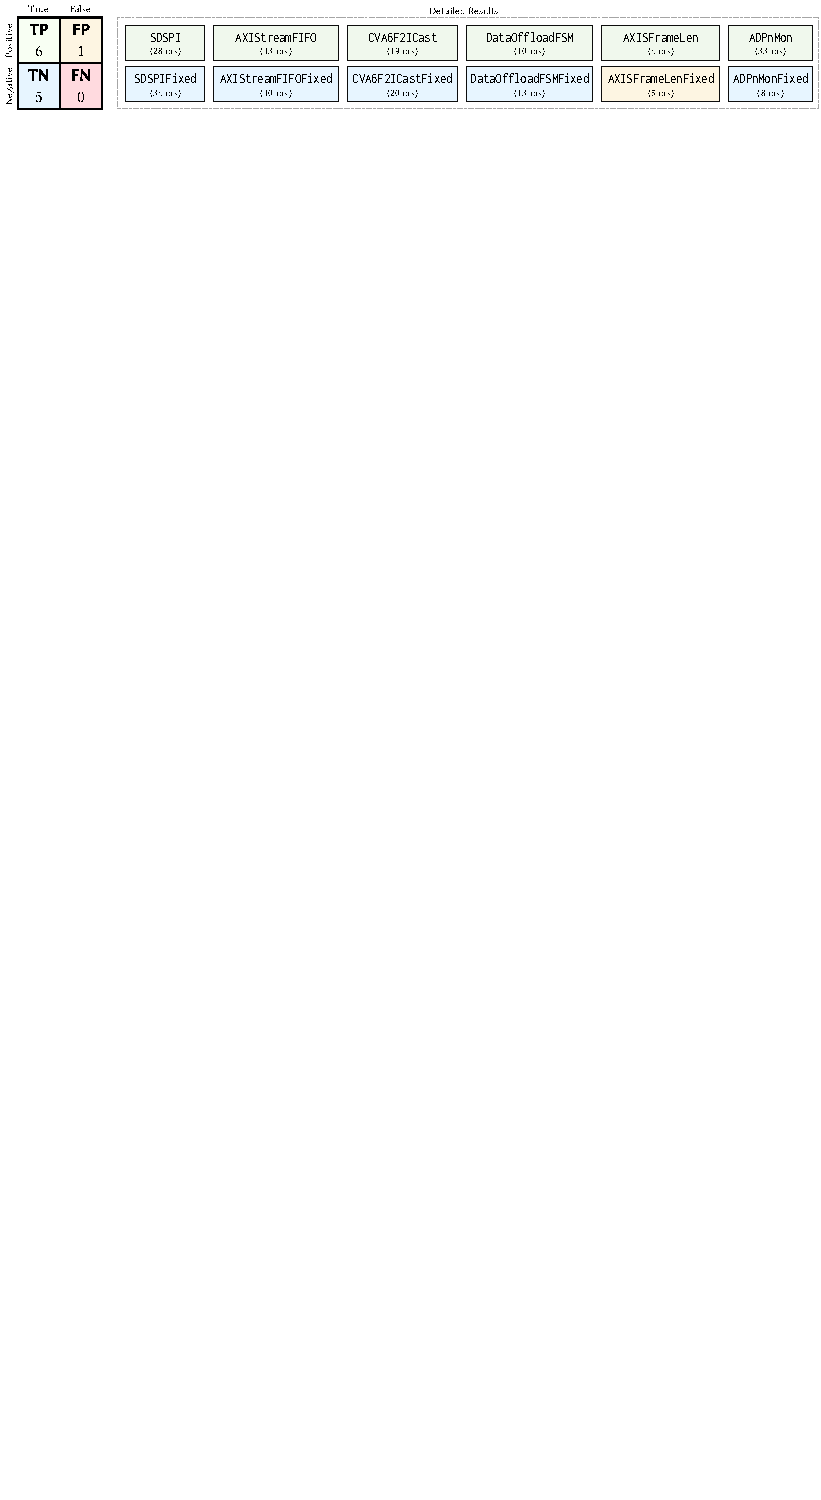
\includegraphics[clip,trim=0 23.5cm 0 0]{figures/asynchrony-eval}
    \caption{Evaluation of signal asynchrony analysis (recall: 100\%, precision: 85.7\%), a hardware bug detection client built on top of \tia; analysis times are shown in parentheses.}\label{fig:eval-asynchrony}
\end{figure}

\paragraph{Benchmarks}
Our signal asynchrony analysis is inspired by a survey of hardware bugs~\cite{ma_debugging_2022}, which defines signal asynchrony bugs and reproduces two such bugs from bug-fixing commits in open-source hardware projects: an SD card controller (\texttt{SDSPI}~\cite{sdspi}) and an AXI4-stream FIFO (\texttt{AXIStreamFIFO}~\cite{axi-stream-fifo}).
We use both the buggy and corresponding fixed versions of these two designs as benchmarks, yielding four benchmarks in the dashed box in Figure~\ref{fig:eval-asynchrony};
the fixed versions are denoted by appending the \texttt{Fixed} suffix to their original names.

The artifact~\cite{ma_debugging_2022_artifact} accompanying the survey~\cite{ma_debugging_2022} additionally lists eight signal asynchrony bug-fixing commits but does not provide proof-of-concept tests to reproduce their buggy behavior.
We attempted to reproduce these bugs and successfully developed proof-of-concept tests for four of them:
a floating-point unit (FPU) component (\texttt{CVA6F2ICast}~\cite{cva6-f2i-cast}),
a storage unit access controller (\texttt{DaraOffloadFSM}~\cite{data-offload-fsm}),
a network interface controller component for frame monitoring (\texttt{AXISFrameLen}~\cite{axis-frame-len}), and
a pseudo-random number monitor (\texttt{ADPnMon}~\cite{ad-pn-mon}).
Together with their corresponding fixed versions, these four buggy designs yield eight additional benchmarks, also shown in the dashed box in Figure~\ref{fig:eval-asynchrony}.

For the remaining four bug-fixing commits listed in the artifact~\cite{ma_debugging_2022_artifact}, our investigation found that three are outside the scope of the signal asynchrony bugs defined by the survey.
The remaining commit modifies 68 files, and we could not identify a reproducible signal asynchrony bug from it.

\paragraph{Understanding the Results}
The left part of Figure~\ref{fig:eval-asynchrony} summarizes the overall results of signal asynchrony analysis, while the right part details the results for each benchmark, with colors indicating the classification.
There are 6 true positives (TPs, in green), where our analysis correctly identifies buggy designs as buggy, and 5 true negatives (TNs, in blue), where it correctly identifies non-buggy designs as non-buggy.
There are no false negatives (FNs, in red), where our analysis fails to detect a true asynchrony bug, yielding a recall of $\mathit{recall} = \mathit{TP}/(\mathit{TP}+\mathit{FN}) = 100\%$.
There is only one false positive (FP, in yellow), where our analysis reports a asynchrony bug in a non-buggy design, yielding a precision of $\mathit{precision} = \mathit{TP}/(\mathit{TP}+\mathit{FP}) = 85.7\%$.

The false positive occurs in \texttt{AXISFrameLenFixed}.
This module expects its AXI monitor interface inputs to follow a specific protocol, under which its outputs \texttt{frameLen} and \texttt{frameLenValid} are synchronized by the input \texttt{monitorAxisTlast}.
However, our analysis does not incorporate this input constraint and therefore considers these outputs potentially asynchronous under unconstrained inputs.
Thus, although the bug is fixed under the module's intended input protocol, our analysis reports a potential asynchrony under unconstrained inputs, resulting in the false positive.

As indicated by the analysis times in parentheses under the benchmark names in Figure~\ref{fig:eval-asynchrony}, our signal asynchrony analysis is also efficient, taking an average of 16.4 milliseconds across the benchmarks, including the time spent by the underlying \tia.
This efficiency stems from both the efficiency of \tia and the lightweight reuse of its computed temporal influence information: the client analysis only queries \tia's results to check signal synchronization, as described in Section~\ref{sec:client-asynchrony}, and therefore incurs little additional computational overhead.
